\documentclass{../template/Report}%方括号内写yuxi即生成预习报告\documentclass[yuxi]{../template/Report}
\settemplatedir{../template/}%设置模板路径
\exname{} %实验名称
\extable{} %实验桌号
\instructor{} %指导教师
\class{} %班级
\name{} %姓名
\stuid{} %学号

\nyear{} %年
\nmonth{} %月
\nday{} %日
\nweekday{} %星期几,e.g. \nweekday{三}
\daypart{}%上午/下午

\redate{} %如有实验补做,补做日期
\resitu{} %情况说明:

\begin{document}
\maketitle%输出封面
\section{预习测试(10分)}
上课前到学在浙大上完成,注意测试仅1次机会。期末时测试分数会与报告其它部分的分数进行加和处理。
\section{原始数据(20分)}
\begin{figure}[H]
  \centering
  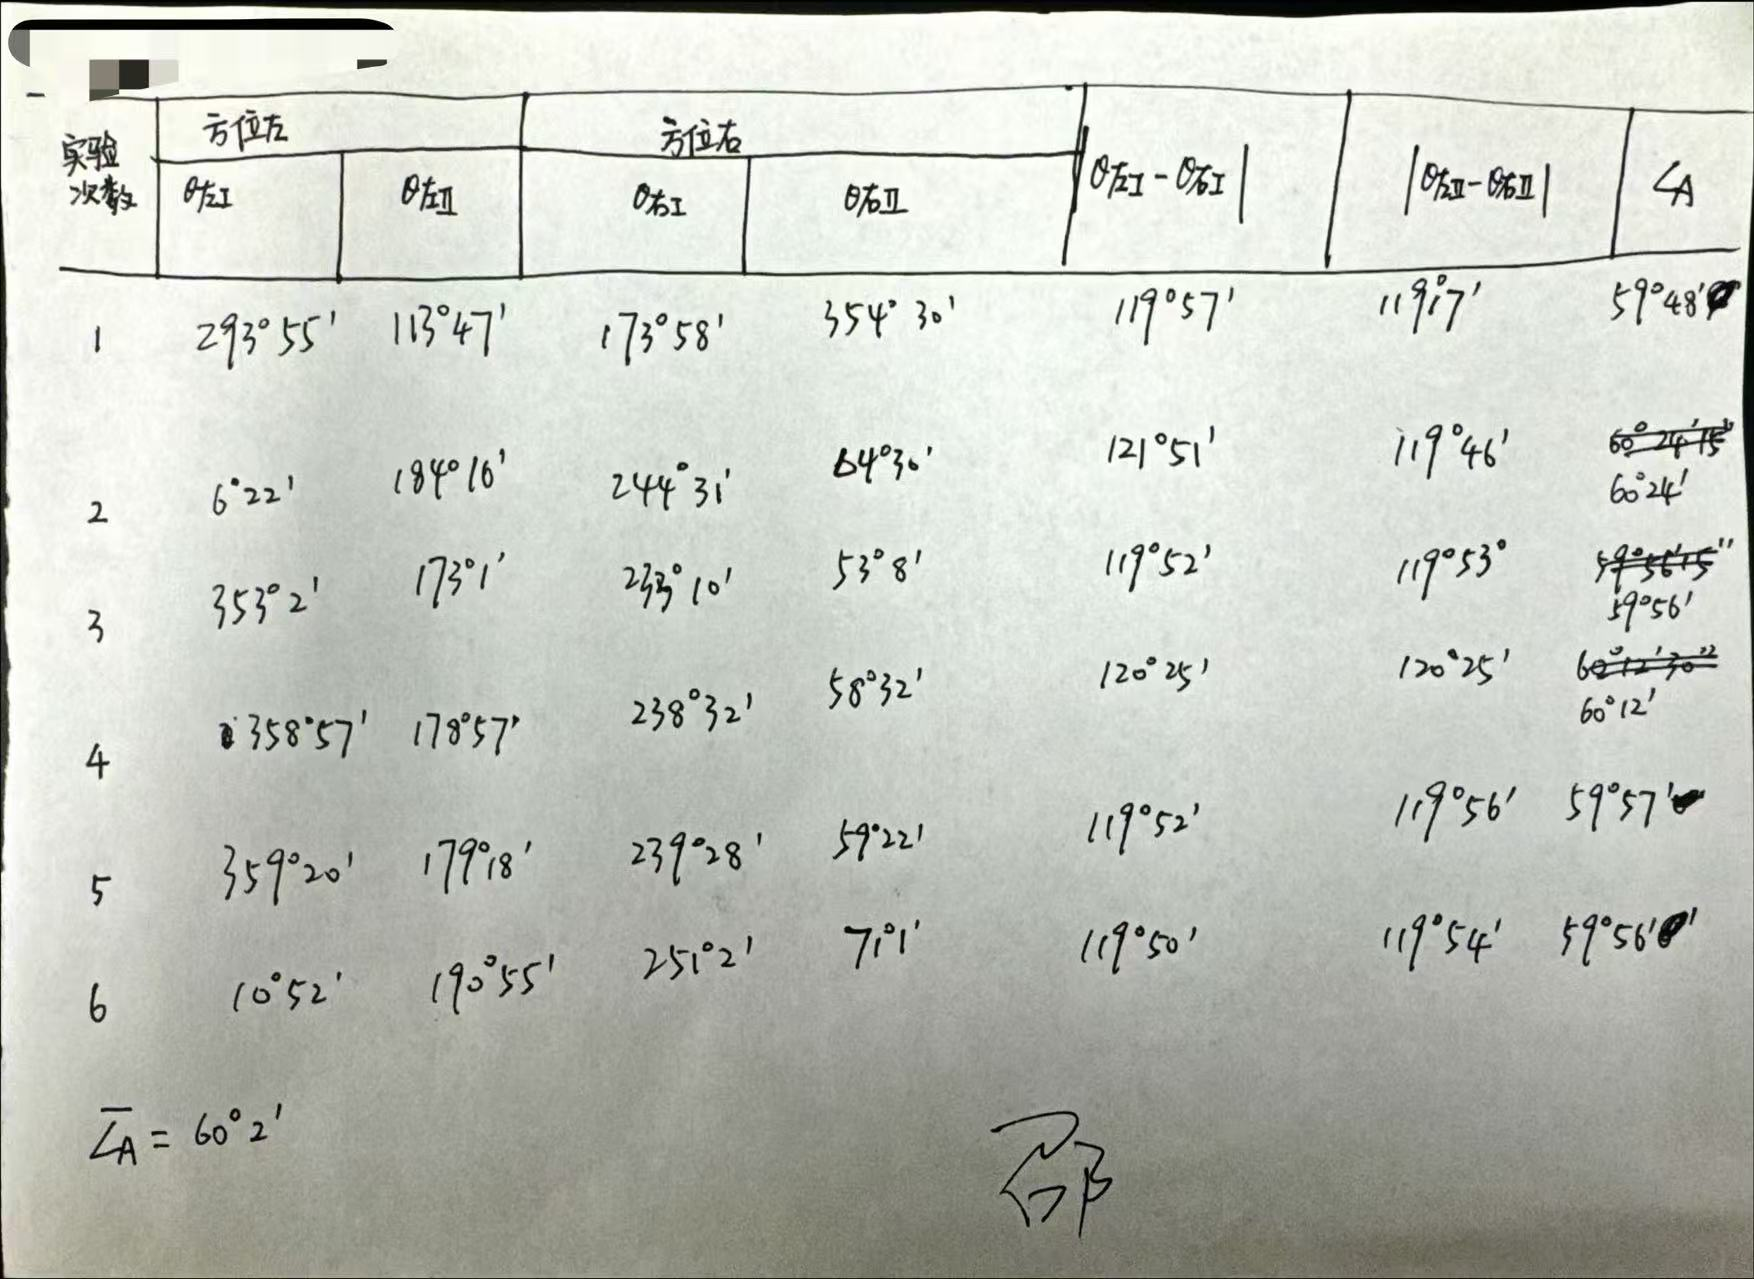
\includegraphics[width=.9\textwidth]{./figures/数据.jpg}
  \caption{原始数据}
\end{figure}
\section{结果与分析}
\subsection{数据处理与结果(30分)}
\begin{table}[H]
\centering
\caption{数据处理与结果}
\label{tab:data}
\resizebox{.95\textwidth}{!}{
\begin{tabular}{|l|cc|cc|c|c|c|}
\hline
\multirow{2}{*}{\begin{tabular}[c]{@{}l@{}}实验\\ 次数\end{tabular}} &
  \multicolumn{2}{c|}{方位左} &
  \multicolumn{2}{c|}{方位右} &
  \multirow{2}{*}{$\left|\theta_\text{左I} - \theta_\text{右I}\right|$} &
  \multicolumn{1}{l|}{\multirow{2}{*}{$\left|\theta_\text{左II} - \theta_\text{右II}\right|$}} &
  \multicolumn{1}{l|}{\multirow{2}{*}{$\angle A$}} \\ \cline{2-5}
 &
  \multicolumn{1}{c|}{\begin{tabular}[c]{@{}c@{}}游标I窗\\ $\theta_\text{左I}$\end{tabular}} &
  \begin{tabular}[c]{@{}c@{}}游标II窗\\ $\theta_\text{左II}$\end{tabular} &
  \multicolumn{1}{c|}{\begin{tabular}[c]{@{}c@{}}游标I窗\\ $\theta_\text{右I}$\end{tabular}} &
  \begin{tabular}[c]{@{}c@{}}游标II窗\\ $\theta_\text{右II}$\end{tabular} &
   &
  \multicolumn{1}{l|}{} &
  \multicolumn{1}{l|}{} \\ \hline
1 & \multicolumn{1}{c|}{\ang{293;55}} & \ang{113;47} & \multicolumn{1}{c|}{\ang{173;58}} & \ang{354;30} & \ang{119;57} & \ang{117;17} & \ang{59;48} \\ \hline
2 & \multicolumn{1}{c|}{\ang{6;22}}   & \ang{184;16} & \multicolumn{1}{c|}{\ang{244;31}} & \ang{64;30}  & \ang{121;51} & \ang{119;46} & \ang{60;24} \\ \hline
3 & \multicolumn{1}{c|}{\ang{353;2}}  & \ang{173;1}  & \multicolumn{1}{c|}{\ang{233;10}} & \ang{53;8}   & \ang{119;52} & \ang{119;53} & \ang{59;56} \\ \hline
4 & \multicolumn{1}{c|}{\ang{358;57}} & \ang{178;57} & \multicolumn{1}{c|}{\ang{238;32}} & \ang{58;32}  & \ang{120;25} & \ang{120;25} & \ang{60;12} \\ \hline
5 & \multicolumn{1}{c|}{\ang{359;20}} & \ang{179;18} & \multicolumn{1}{c|}{\ang{239;28}} & \ang{59;22}  & \ang{119;52} & \ang{119;56} & \ang{59;57} \\ \hline
6 & \multicolumn{1}{c|}{\ang{10;52}}  & \ang{190;55} & \multicolumn{1}{c|}{\ang{251;2}}  & \ang{71;1}   & \ang{119;50} & \ang{119;54} & \ang{59;56} \\ \hline
\end{tabular}
}
\end{table}
$\angle A$平均值:$\bar{\angle A}$ = $\dfrac{\displaystyle\sum_{i=1}^6 \angle A_i}{6} = \ang{60;2}$
\subsection{误差分析(20分)}
(运用测量误差、相对误差或不确定度等分析实验结果,写出完整的结果表达式,并分析误差原因。)
\paragraph{A类不确定度:}
如果有$n$组数据,则A类不确定度的计算方法为:
\[
u_A = \sqrt{\dfrac{1}{n \cdot (n - 1)} \cdot \sum_{i = 1}^n (x_i - \bar{x})^2}
\]
带入数据
\[
u_A = \sqrt{\frac{1}{6 \cdot (6 - 1)} \cdot \left[(\ang{59;48} - \ang{60;2})^2 + \cdots + (\ang{60;12} - \ang{60;2})^2\right]} = \ang{;5.4;}
\]
\paragraph{B类不确定度:}
因为游标读数估计误差为$\pm\ang{0;1}$,故B类不确定度为
\[
u_B = \frac{\Delta_\text{仪}}{\sqrt{3}} = \frac{1}{\sqrt{3}}\ang{;1} = \ang{;0.6;}
\]
\paragraph{合成不确定度:}
\[
u = \sqrt{u_A^2 + u_B^2} = \sqrt{\ang{;5.4;}^2 + \ang{;0.6;}^2} = \ang{;5;}
\]
\paragraph{最终结果表达式}
\[\angle A = \ang{60;2} \pm \ang{;5;}\]
\setlist[enumerate]{leftmargin=6em}
\paragraph{误差原因分析:}
\begin{enumerate}[label=原因\zhnum*:]
    \item \textbf{偏心误差}

    由于望远镜、平行光管的光轴不一定通过分光计的中心轴,刻度盘和游标的中心也不一定在中心轴上,造成读数误差。
    但我们通过读取两个游标视窗的值取平均消除了可能存在的偏心误差。
    \item \textbf{仪器可能存在的误差}

    如仪器老化、刻度不准、仪器热胀冷缩等
    \item \textbf{读数误差}

    由于游标读数的估计误差为$\pm\ang{0;1}$,所以每次读数都会带来一定的误差。而且人为判定狭缝是否处在中心分划板上也会带来读数误差。

    \item \textbf{视差误差}

    在调节望远镜时,如果来自平行光管的狭缝像没有准确地成像在望远镜的十字分划板所在的平面上,就会产生视差误差。

\end{enumerate}
\subsection{实验探讨(10分)}
本实验的核心是分光计的精确调整与棱镜角度的测量。

首先,对分光计进行系统调整,确保:
望远镜聚焦于无穷远且无视差;
通过调整载物台,目镜和平行光管,使得望远镜、平行光管光轴及载物台平面均与仪器中心转轴垂直。

调整完毕后,采用反射法测量棱镜顶角$\alpha$。
将顶角正对平行光管,转动望远镜分别接收并对准由顶角两个反射面反射回来的光线,记下两个位置的角度读数。
这两个读数之差$\beta$是反射光线夹角,
而棱镜顶角恰好为该夹角的一半,即$\alpha = \frac{\beta}{2}$。
\section{思考题(10分)}
\subsection{测量三棱镜顶角时,棱镜摆放的位置怎么选,有区别吗?}
棱镜应该摆放在载物台中间偏上一些的位置,棱镜不同的位置对实验成功与否有一定的影响。
\begin{figure}[H]
\centering
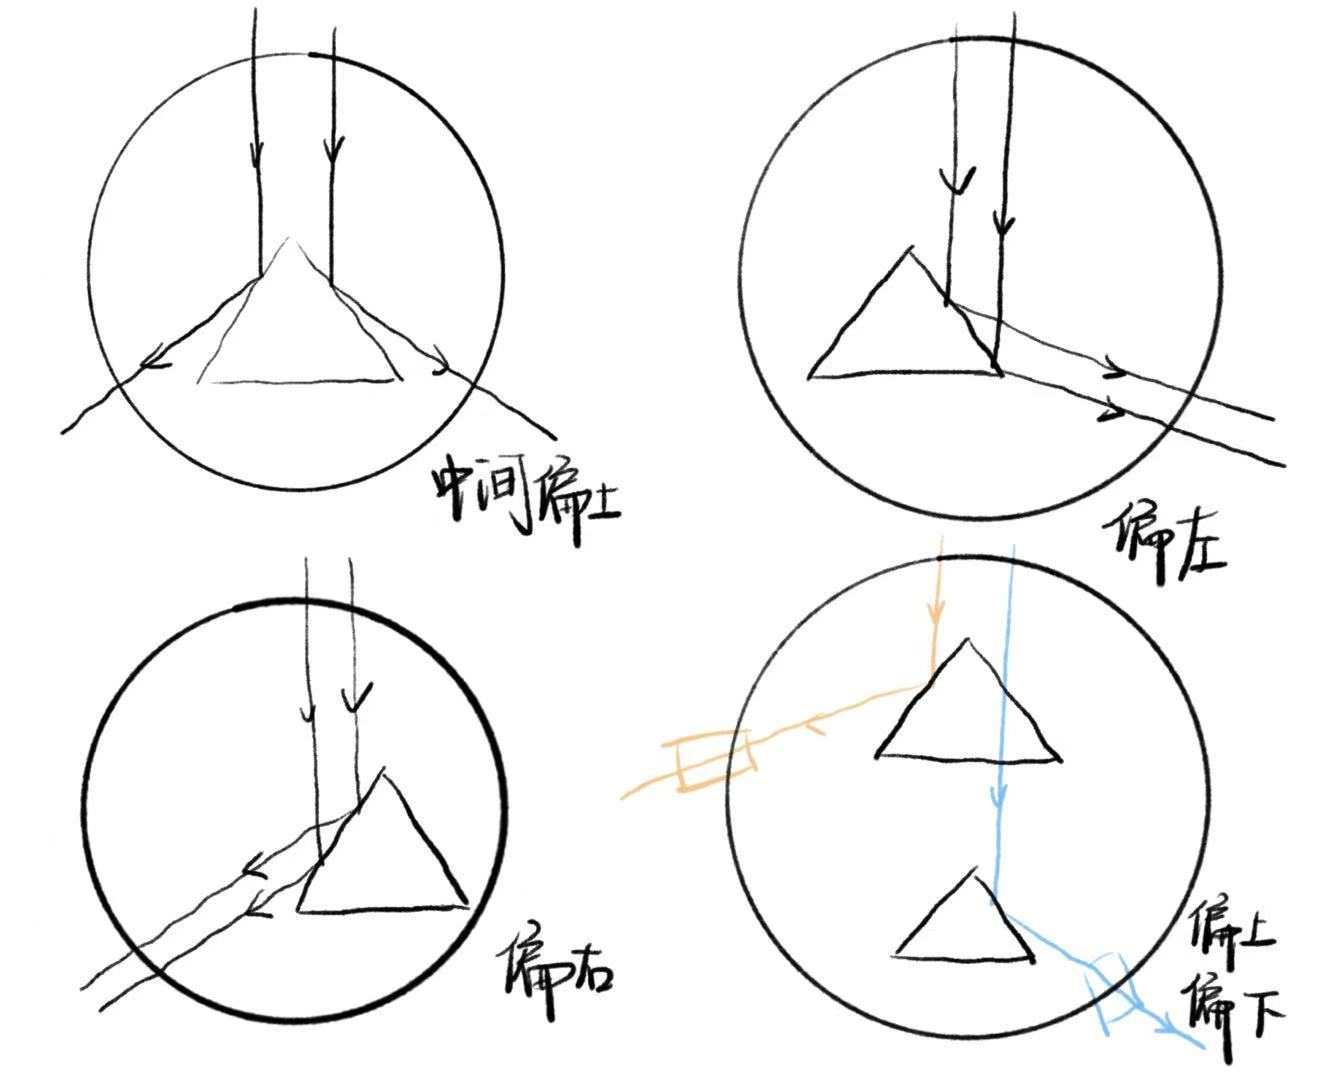
\includegraphics[width=0.9\textwidth]{./figures/思考1.jpg}
\caption{不同的摆放对光路的影响}
\end{figure}
\begin{enumerate}
  \item 三棱镜顶角中间偏上,望远镜可以观察到清晰的狭缝
  \item 三棱镜顶角偏向一边,平行光可能全部在一个反射面反射,另一边看不到反射光,也就无法测量三棱镜顶角
  \item 三棱镜顶角偏前或偏后,则望远镜难以观察到反射光,影响实验效果
\end{enumerate}
\subsection{为什么狭缝要调至适当宽度(\si{1-2}{mm})?太宽,太窄有什么问题?}
\begin{enumerate}
  \item 狭缝太窄:因为三棱镜反射率并不是1,反射之后狭缝亮度会有下降,如果狭缝太窄,那么可能无法观测到平行光反射之后的位置,影响实验效果
  \item 狭缝太宽:无法判断狭缝是否准确落在望远镜中央十字分划板上,无法准确确定望远镜位置,也就没办法准确测量出反射光的角度
\end{enumerate}
  \subsection{粗调时,为什么会出现一面有十字像,转了\ang{180}后没有十字像?这时该如何调节,请简要描述。}
\paragraph{原因} 平台和望远镜可能经过粗调之后可能同时向同个方向倾斜,一开始可能望远镜光轴与平面镜垂直,望远镜中可以看到绿色十字像,但是旋转\ang{180}之后两者倾斜
方向不相同,绿色十字像被反射到视野之外,就无法观察到十字像。
\paragraph{调整方法}
\begin{enumerate}
  \item 可在距离分光计较远处目测分光计望远镜光轴、
  载物盘盘面是否垂直于中心转轴,
  特别是可通过一定的速度旋转游标盘(带动载物盘旋转),
  观察载物盘与载物台间的缝隙宽度是否相同,
  如果载物台是倾斜的,在旋转时可以感受到载物台与水平面间距在变化,
  进而判断载物盘盘面是否大致垂直中心转轴,
  并利用载物盘下方的3个旋钮进行调整。
  \item 可直接在望远镜光轴附近(上方或下方,不是从望远镜目镜筒中观察)直接观察从平面镜或三棱镜表面上反射回来的像的位置,
  判断反射光线高于还是低于望远镜筒,并进行调节
  \item 等经过粗调之后望远镜筒中出现了两个上下错开的像之后,再通过调整载物台旋钮把其中一个像调整到两个像位置的中间,
  并不断调整,直至两个像完全重合
  \item 重复两次调整完载物台三个旋钮后,再调整望远镜俯仰角,使得绿色十字像处在分划板中心
\end{enumerate}
\subsection{你可以用别的方法测量三棱镜顶角吗?}
\paragraph{激光反射法}
\textbf{原理:}利用光的反射定律。一束光线射向顶角两侧的面,两束反射光线之间的夹角是顶角的两倍。
所需设备:激光器、三棱镜、一个大的屏幕或墙壁、卷尺。

\textbf{步骤:}

\begin{enumerate}[label=\textbf{Step }\arabic{*}.]
  \item 将三棱镜放在桌子上,顶角$\alpha$朝向激光器。
  \item 调整激光器,使其光束正好射在三棱镜的顶角棱线上,这样光束会同时照射到两个侧面。
  \item 在三棱镜后方放置一个垂直的屏幕,您会看到两个反射回来的光斑。
  \item 测量三棱镜顶角到屏幕的垂直距离$L$。
  \item 测量屏幕上两个光斑之间的距离$d$。
\end{enumerate}

\textbf{计算:}
两束反射光线之间的夹角$\beta$可以通过三角函数计算得出。从图中可以看出,$ \tan(\frac{\beta}{2}) = \frac{d/2}{L} $。
再根据反射定律可以证明,这两束反射光线之间的夹角$\beta$等于顶角$\alpha$的两倍,即$\alpha = \frac{\beta}{2}$。
因此:
\[
\alpha = \arctan(\frac{d}{2L})
\]
\insertnotes
\end{document}